% subsection: 特性方程式型 \, $a_{n+1}=pa_n+q$

  \subsection{特性方程式型 \, $a_{n+1}=pa_n+q$}
    応用パターンの1つ目,特性方程式型について説明する.
    まずは一般的な形を見せよう.
    \[
      a_{n+1}=pa_n+q
    \]
    さて,この漸化式はどのように解くことができるだろうか.
    数学の問題を解くときの強い原則は,知っている形にすることである.
    ここでも同じで,漸化式をうまく変形して知っている形に変形できれば解くことができる.
    
    そこから考えて,先に扱った基本4パターンの知識を使ってこの漸化式を分析してみよう.
    この漸化式は$a_n$に対して$p$が掛けられ,さらに$q$が足されている.
    つまり,この漸化式は,等比型と階差型の組み合わせからなっていることがわかる.
    そこから判断して,ここは少々突飛な発想ではあるが,この漸化式を等比型に帰着させることを試みよう.
    
    この漸化式は,等比型漸化式
    \[
      a_{n+1}=pa_n
    \]
    に対して$q$が足されたものだ.
    つまりは,\,$q$がうまく消えてくれるような計算式を考えたいのだ.
    その分だけうまく戻せばよい.
    結論から言えば,
    \[
      \begin{array}{rrl}
         & a_{n+1}={} & pa_n+q\\
        -\,) & \alpha={} & p\alpha+q\\ \hline
         & a_{n+1}-\alpha={} & p(a_n-\alpha)
      \end{array}
    \]
    より,
    \[
      a_{n+1}-\alpha=p(a_n-\alpha)
    \]
    を満たすような$\alpha$を考えればよい.
    この式を特性方程式と言う.
    形式的には,
    \[
      a_{n+1}-\alpha=p(a_n-\alpha)
    \]
    または
    \[
      \alpha=p\alpha+q
    \]
    を解き,\,$\alpha$を求めればよい.
    続けると,
    \begin{align*}
      &a_{n+1}-\alpha=p(a_n-\alpha)\\
      &a_{n+1}-\alpha=pa_n-p\alpha\\
      &a_{n+1}=pa_n-p\alpha+\alpha\\
      &a_{n+1}=pa_n+(1-p)\alpha
    \end{align*}
    $(1-p)\alpha$について,
    \[
      a_{n+1}=pa_n+q
    \]
    と係数比較を行うと,
    \begin{align*}
      &q=(1-p)\alpha\\
      &\therefore \quad \alpha=\frac{q}{1-p}
    \end{align*}
    $\alpha$が求まったので,次のステップに移る.
    式の見た目を整えるために,\,$b_n=a_n-\alpha$と置く.
    すると,
    \begin{align*}
      &a_{n+1}-\alpha=p(a_n-\alpha) \iff b_{n+1}=pb_n
    \end{align*}
    この等比型漸化式$b_{n+1}=pb_n$を解くと,
    \begin{align*}
      &b_{n+1}=pb_n\\
      &\therefore \quad b_n=b_1p^{n-1}\\
      &a_n-\alpha=(a_1-\alpha)p^{n-1}\\
      &a_n=(a_1-\alpha)p^{n-1}+\alpha\\
      &\therefore \quad a_n=\left(a_1-\frac{q}{1-p}\right)p^{n-1}+\frac{q}{1-p}
    \end{align*}
    となり,\,$a_n$の一般項が示された.
    やってほしくないことは,この議論の末に得られた結果の形だけを覚えて問題に挑むことである.
    この議論全体を問題を解くたびに都度再現してほしい.

    もう少し数学の世界に深入りしていこう.
    \,$\alpha$を求めるというのはどういった意味合いを持つだろうか.
    漸化式を
    \[
      a_{n+1}=f(a_n)
    \]
    と考え,
    \[
      y=f(x)=px+q
    \]
    について,\,$y=x$との交点,すなわち
    \[
      f(a_{n+1})=f(a_n)
    \]
    を満たすような不動点を考える.図示すると

    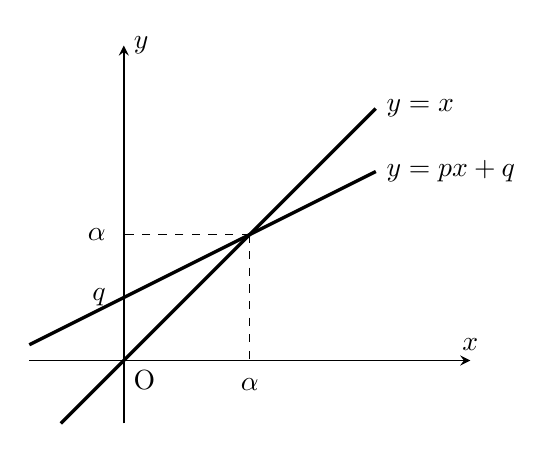
\begin{tikzpicture}[scale=0.8]
      \draw[->,>=stealth,semithick] (-1.5,0)--(5.5,0)node[above]{$x$};
      \draw[->,>=stealth,semithick] (0,-1)--(0,5)node[right]{$y$};
      \draw (0,0)node[below right]{O};

      \draw[very thick,domain=-1:4]
        plot(\x,\x)node[right]{$y=x$};

      \draw[very thick,domain=-1.5:4]
        plot(\x,\x/2+1) node[right] {$y=px+q$};

      % q
      \node[left=3pt] at (0,1) {$q$};

      % 交点から各軸へ点線
      \draw[dashed] (2,2) -- (2,0);
      \draw[dashed] (2,2) -- (0,2);

      % α
      \node[below=3pt] at (2,0) {$\alpha$};
      \node[left=3pt] at (0,2) {$\alpha$};
    \end{tikzpicture}

    というような状況である.
    この交点$(\alpha,\alpha)$を原点と思ってグラフをみると,この座標平面は$y=px$と$y=x$のグラフが原点から始まって進んでいくようなものに見える.
    言い換えれば等比型漸化式に帰着させたということである.
    このような点$(\alpha,\alpha)$を不動点という.

    この不動点を知ることによって,複雑な値の変化をより簡素な値の変化に置き換えることができる.
    また,この話から,漸化式の作る値はのおよその大きさは,\,$p$が作るということが分かる.
    \,$a_n$に対しての和で影響を与える$q$によってもたらされる値の変化より,\,$a_n$に対して積で影響を与える$p$によってもたらされる値の変化の方がはるかに大きいからだ.

    また,特性方程式型漸化式には別の解法が存在する.
    以下に示す.
    \begin{align*}
      &a_{n+1}=pa_n+q \tag*{\(\cdots\) (1)}\\
      &a_{n+2}=pa_{n+1}+q \tag*{\(\cdots\) (2)}\\
    \end{align*}
    $(2)-(1)$をし
    \[
      a_{n+2}-a_{n+1}=p(a_{n+1}-a_n)
    \]
    ここで,\,$b_n=a_{n+1}-a_n$と置くと,
    \begin{align*}
      &b_{n+1}=pb_n
    \end{align*}
    このようにすることで,漸化式は等比数列に帰着する.
    この後の処理は読者に委ねる.

    こちらの図形的解釈は先程の交点を考えるものとは違い,今度は平行な直線を考えることに該当する.
    先程の議論から,\,$p$の情報が欠けた式はその漸化式から生まれる一般項の様相を大きく変えてしまうことがわかる.
    したがってこの場合では$y=x$の代わりに$y=px$を用いる.
    これらの前提を元に図示すると

    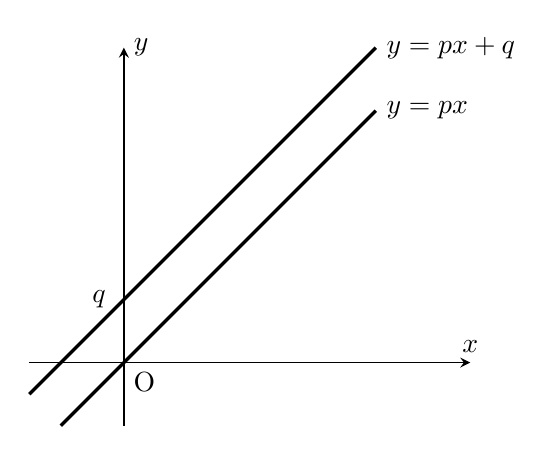
\begin{tikzpicture}[scale=0.8]
      \draw[->,>=stealth,semithick] (-1.5,0)--(5.5,0)node[above]{$x$};
      \draw[->,>=stealth,semithick] (0,-1)--(0,5)node[right]{$y$};
      \draw (0,0)node[below right]{O};

      \draw[very thick,domain=-1:4]
        plot(\x,\x)node[right]{$y=px$};

      \draw[very thick,domain=-1.5:4]
        plot(\x,\x+1) node[right] {$y=px+q$};

      % q
      \node[left=3pt] at (0,1) {$q$};

    \end{tikzpicture}
    
    常に関数の差が$q$と一定になっていることが図からわかる.

    今後,特性方程式を用いた解法を多数扱う.
    特性方程式は漸化式を解く中で重要な概念なのである.
    その背景には行列や線形代数が深く絡んでいる.

  \noindent \textbf{【例題】}
  \begin{enumerate}[label=(\arabic*),parsep=3pt]
    \item $\displaystyle a_1=1,\, a_{n+1}=2a_n+1$
    \item $\displaystyle a_1=1,\, a_{n+1}=\frac{1}{2}a_n+2$
    \item $\displaystyle a_1=1,\, a_{n+1}=a_n+2$
  \end{enumerate}

  \noindent\textbf{【方針】}
  \begin{enumerate}[label=(\arabic*),parsep=3pt]
    \item まずは,\,$\alpha$を求めて等比型に帰着させる方法で解きましょう.
    \item 同じく,\,$\alpha$を求めて等比型に帰着させる方法で解きましょう.
    \item この漸化式は等差型ですが,試しに特性方程式型に帰着させることを考えてみましょう.\,$\alpha$は存在しますか?
  \end{enumerate}

  \noindent\textbf{【解答】}
  \begin{enumerate}[label=(\arabic*),parsep=3pt]
    \item $\displaystyle a_n=2^n-1$
    \item $\displaystyle a_n=4-3\cdot\left(\frac{1}{2}\right)^{n-1}$
    \item $\displaystyle a_n=1+2(n-1)$
  \end{enumerate}

  \noindent\textbf{【解法】}
  \begin{enumerate}[label=(\arabic*),parsep=3pt]
    \item $\displaystyle a_1=1,\,a_{n+1}=2a_n+1$\\
          特性方程式を考えると,
          \[
            \alpha=2\alpha+1
            \quad\Longleftrightarrow\quad
            \alpha=-1
          \]
          である.

          $b_n=a_n-\alpha=a_n+1$とおくと,
          \begin{align*}
            b_{n+1}
              &=a_{n+1}+1\\
              &=2a_n+2\\
              &=2(a_n+1)\\
              &=2b_n.
          \end{align*}
          また,\,$b_1=a_1+1=2$であるから,
          \[
            b_n=2^n.
          \]
          よって,
          \[
            a_n=b_n-1=2^n-1.
          \]

    \item $\displaystyle a_1=1,\,a_{n+1}=\frac12a_n+2$\\
            特性方程式を考えると,
            \[
              \alpha=\frac12\alpha+2
              \quad\Longleftrightarrow\quad
              \alpha=4
            \]
            である.

            $b_n=a_n-\alpha=a_n-4$とおくと,
            \begin{align*}
              b_{n+1}
                &=a_{n+1}-4\\
                &=\frac12a_n+2-4\\
                &=\frac12(a_n-4)\\
                &=\frac12b_n.
            \end{align*}
            また,\,$b_1=a_1-4=-3$であるから,
            \[
              b_n=-3\left(\frac12\right)^{n-1}.
            \]
            よって,
            \[
              a_n=b_n+4
              =4-3\left(\frac12\right)^{n-1}.
            \]
     \item $\displaystyle a_1=1,\, a_{n+1}=a_n+2$\\
           $\alpha$は存在しないので,特性方程式型に帰着させることはできない.
           これが意味することは,不動点を持たないということである.
  \end{enumerate}

